% This work by Jeremy A. Hansen is licensed under a Creative Commons 
% Attribution-NonCommercial-ShareAlike 3.0 Unported License, 
% as described at http://creativecommons.org/licenses/by-nc-sa/3.0/legalcode

An array is a series of variables that are the same of the same type (\Code{int}, \Code{float}, \Code{double}, \Code{char}, and so on).
Arrays are held in a computer's memory in a strict linear sequence.
An array does not hold anything other than the elements of the specified type, so there is no assigning an array of type \Code{float} and hoping to store a \Code{string} there. 
Doing so would cause a ``type mismatch error'' and the program wouldn't compile. 
To create an array, the programmer types something like this:

\noindent\begin{minipage}{\linewidth}\begin{lstlisting}
char Scott[5];
\end{lstlisting}\end{minipage}

The \Code{char} is the data type for all elements in the array, \Code{Scott} is the name of the array (you can be as creative as you want with the name), and the 5 inside the square brackets represents the size of the array. 
So \Code{char Scott[5]} can hold 5 pieces of data that are of type \Code{char}. 

\begin{figure}[tbh]
  \centering
  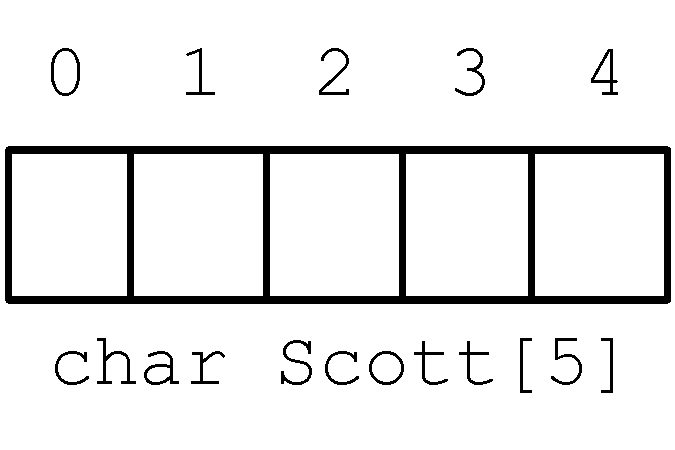
\includegraphics[width=0.6\textwidth]{diagrams/array-diagram-1.pdf}
  \caption{The array named \Code{Scott} has five spaces for \Code{char} data} \label{fig:array-diagram-1}
\end{figure}

When trying to visualize an array, think of a rectangle split up into as many pieces as the array has places to hold data.
In Figure \ref{fig:array-diagram-1}, the rectangle has five spaces, each of type \Code{char} awaiting some values. 

In order to refer to the individual elements in an array, we start with the number 0 and count upwards. 
We use \Code{[0]} to access the first element in the array, \Code{[1]} for the second, \Code{[2]} for the third, and so on. 
In order to read or write certain locations of the array, we state the name of the array and the element we want to access. 
It should look like this:

\noindent\begin{minipage}{\linewidth}\begin{lstlisting}
Scott[3] = 'Q';
cout << Scott[3];
\end{lstlisting}\end{minipage}

The diagram below depicts how the computer interprets this. \nopagebreak[4]

\begin{figure}[tbh]
  \centering
  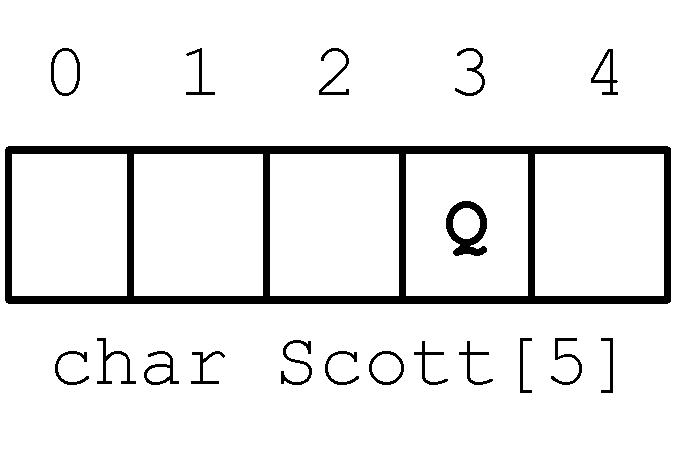
\includegraphics[width=0.6\textwidth]{diagrams/array-diagram-2.pdf}
  \caption{The fourth element of \Code{Scott} now contains \Code{'Q'}} \label{fig:array-diagram-2}
\end{figure}


You can also store values inside the array ahead of time when you declare the array. 
To do so, you need to enclose the values of the appropriate type in brackets and separate the values with a comma. 
Below are two examples, one an array where each element is of type \Code{char} and another where each element is of type \Code{int}.

\noindent\begin{minipage}{\linewidth}\begin{lstlisting}
char Scott[5] = {'S', 'c', 'o', 't', 't'};	
int John[5] = {99, 5, 1, 22, 7};
\end{lstlisting}\end{minipage}
	
Note that, in the C and C++ language, arrays of characters intended to be treated as a string must contain a special character called the \Keyword{null character}\footnote{Often abbreviated NUL; Note that this is not the same as the NULL pointer described in Chapter \ref{chap_pointers}.} or \Keyword{null terminator}. 
The null terminator marks the end of the string. 
In C++, this is represented by the special character \Code{'\textbackslash0'}. 
Because the null temrinator takes up one element in the array, any character array that is intended to be used as a printable string must be declared having a size one larger than the longest string that you expect to store. 
Initializing the above character array should really be done as the following (notice that we make the array one element larger!):

\noindent\begin{minipage}{\linewidth}\begin{lstlisting}
char Scott[6] = {'S', 'c', 'o', 't', 't', '\0'};	
\end{lstlisting}\end{minipage}

Alternatively, you can initialize a character array with a string literal, as below. 
We discuss string literals in more detail in Chapter \ref{chap_constants}.

\noindent\begin{minipage}{\linewidth}\begin{lstlisting}
char Scott[6] = "Scott";	
\end{lstlisting}\end{minipage}

It is also possible to let the computer figure out the appropriate length for an array when the array is being initialized at the same time as when it is declared. 
The below code produces an identical array as the previous example:

\noindent\begin{minipage}{\linewidth}\begin{lstlisting}
char Scott[] = "Scott";	
\end{lstlisting}\end{minipage}

\LevelD{Multi-dimensional Arrays}

A two-dimensional array (some might call it a ``matrix'') is the same thing as an array, but is an ``array of arrays''.
Here's a two-dimensional three-by-three array:

\noindent\begin{minipage}{\linewidth}\begin{lstlisting}
int Rich[3][3]; // 2D
\end{lstlisting}\end{minipage}

Declaring arrays with more dimensions are possible with similar syntax. 
Here's a three-dimensional $10\times10\times10$ example:

\noindent\begin{minipage}{\linewidth}\begin{lstlisting}
int Sam[10][10][10]; // 3D
\end{lstlisting}\end{minipage}

And here is a four-dimensional $10\times10\times10\times10$ array. 
This is possible even though it's hard to visualize.

\noindent\begin{minipage}{\linewidth}\begin{lstlisting}
int Travis[10][10][10][10]; // 4D
\end{lstlisting}\end{minipage}

A user can input values into a multi-dimensional array in a similar way as a single-dimensional array. 

\noindent\begin{minipage}{\linewidth}\begin{lstlisting}
int neo[3][3] = {{1,2,3}, {4,5,6}, {7,8,9}}; 
cout << neo[0][0] << endl << endl; // first number, 1
cout << "  " << neo[2][2]; // last number, 9
\end{lstlisting}\end{minipage}


The same logic is applied for 3-dimensional and 4-dimensional arrays, but when filling them be mindful of the order of the input so that when you want to view certain elements in the array you are able to correctly access them. 

\LevelD{Review Questions}

\begin{enumerate}
	\item Declare an integer array named \Code{myInt} with a size of 10.
  \item If an array has a size of 20, how many indexes are there in the array and what are they?
  \item Declare a character array named \Code{myArray} with a size of 4, and initialize the characters in the array to \Code{'Z'}, \Code{'a'}, \Code{'c'}, and \Code{'h'}. 
  \item 
  Create a program in which an integer array named \Code{myArray} is declared with a size of 10. 
  Use a \Code{for} loop to prompt the user to store a value in every index of the array. 
  After the array is given values, output the values of the array to the screen using a \Code{for} loop. 
  Output each value of the array on its own line.
\end{enumerate}

\LevelD{Review Answers}

\begin{enumerate}
	\item \Code{int myInt[10];}
  \item There are 20: indexes 0 through 19.
  \item \Code{char myArray[4] = {'Z', 'a', 'c', 'h'};}
  \item 
\noindent\begin{minipage}{\linewidth}\begin{lstlisting}
#include <iostream>
using namespace std;
int main()
{
  int myArray[10];
  cout << "Enter 10 integers, press [ENTER] "
    << "after every integer.\n";
  for (int i = 0; i < 10; i++)
  {
    cin >> myArray[i];
  }
  for (int j = 0; j < 10; j++)
  {
    cout << myArray[j] << endl;
  }
  return 0;
}
\end{lstlisting}\end{minipage}
\end{enumerate}

\LevelD{Further Reading}

\begin{itemize}
\item \url{http://www.cplusplus.com/doc/tutorial/arrays/}
\item \url{http://www.cplusplus.com/forum/beginner/43663/}
\item \url{http://msdn.microsoft.com/en-us/library/7wkxxx2e.aspx}
\item \url{https://www.youtube.com/watch?v=SFGOAKYXfOo}
\end{itemize}	